\section{The simulation study: details and further results}
\label{sec:supp-sim}

This section completes Section 5 of the paper.

\subsection*{Test functions}

Before they are centered and scaled to unit norm in $L_2[0,1]$, the two
components of the uneven cell whose scale changes along the interval are
\[
  w(u)\Bigl[\exp\Bigl\{-\frac{(u-0.40)^{2}}{2(0.10)^{2}}\Bigr\}
  - 0.8\exp\Bigl\{-\frac{(u-0.72)^{2}}{2(0.018)^{2}}\Bigr\}\Bigr]
  \quad\text{and}\quad
  w(u)\sin\{2\pi(u + 3.5u^{2})\},
\]
with the window $w(u) = \eta(u/0.08)\,\eta\{(1-u)/0.08\}$, where
$\eta(t) = e^{-1/t}/(e^{-1/t} + e^{-1/(1-t)})$ for $0 < t < 1$,
$\eta(t) = 0$ for $t \le 0$ and $\eta(t) = 1$ for $t \ge 1$. The window equals
one on $[0.08, 0.92]$ and vanishes with all its derivatives at $0$ and $1$, so
that the periodic extensions of the two components are infinitely
differentiable and the cell measures uneven curvature and not a seam at
$0 \equiv 1$. The bumps, blocks and heavisine functions are those of
\citet{Donoho-Johnstone-1994}, with their constants, on $[0,1]$. The
centering and the scaling constants are computed on $2^{16}$ midpoints of
$[0,1]$.

\subsection*{The larger model}

With $(p,q) = (6,4)$ the levels are $(1, 2, -1.5, 0.5, 1, 2)$, and the
nonzero components are $\gcomp{1}{1}$ (bumps), $\gcomp{1}{2}$ (blocks) and
$\gcomp{2}{1}$ (heavisine), as in the inhomogeneous cell, and
$\gcomp{3}{3}$ (bumps), $\gcomp{3}{4}$ (blocks) and $\gcomp{4}{3}$
(heavisine); the coefficients $\beta_5$ and $\beta_6$ are constant. The grid
of $J$ stops at 7, since at $J = 8$ the design has $6 \times 4 \times 255 =
6120$ penalized columns for 1000 observations.

\subsection*{The grids of the splines}

In either search of \texttt{mgcv} a dimension above 80 whose smooths would
have more than $2n$ coefficients is not fitted, which stops the grid at 120 in
the mixed cell at $n = 1000$ and at 80 in the larger model, and a fit by REML
whose smoothing parameters do not converge within 80 outer iterations leaves
the search. At $n = 1000$ the grid of GAM (REML) stops at 160 because the fit
at 240 did not converge in about a third of the replicates of the
inhomogeneous cell, and in two of them did not finish in 15 hours; where it
was fitted, it would lower the error of GAM (REML) by 0.3\% in that cell and
by 1.2\% in the uneven one.

\subsection*{Further results}


Tables~\ref{tab:sim-sizes} to~\ref{tab:sim-sizes-null} give, one cell each,
the errors and the frequency of the exact structure of every row at every
sample size, together with the coordinatewise lasso of Section 4 of the
paper, fitted at the pair chosen by cross-validation (Lasso) and thresholded
by the one standard error rule (Lasso + threshold);
Table~\ref{tab:sim-structure} gives the null blocks kept at $n = 1000$ and
Table~\ref{tab:sim-paired} the paired comparisons; Table~\ref{tab:sim-arms}
the arms at $n = 1000$ and the larger model;
Tables~\ref{tab:sim-tuning} and~\ref{tab:sim-tuning-b} the resolution or
dimension chosen, the fraction of replicates at the top of the grid and the
time; and Table~\ref{tab:sim-slopes} the slope of the logarithm of the mean
squared error against $\log n$.

The coordinatewise lasso with the threshold recovers the same structure as
the WAFC from $n = 1000$, and less often at $n = 500$ in the mixed cell (69\%
against 84\%). Its prediction error is 3\% to 11\% above that of the WAFC in
the inhomogeneous and mixed cells at every sample size and 2\% to 5\% above
it in the uneven cell, within 1\% in the null cell, and in the smooth cell
7\% below it at $n = 250$ and within 4\% at the other sizes; the blocks of
the penalty pay where the components are inhomogeneous. The WAFC reaches the
top of its grid of $J$ in at most 24\% of the replicates of a cell. GAM
(GCV), whose grid is not extended because of the cost of its fits, chooses
its top in at least 99\% of the replicates of the inhomogeneous cell from
$n = 500$. GAM (REML) chooses the top of its grid in 71\% and 65\% of the
replicates of the inhomogeneous and mixed cells at $n = 500$, where the grid
stops at 80, in 16\% and 97\% at $n = 1000$, where the size rule stops it at
120 in the mixed cell, and in every replicate of both at $n = 2000$. The time
of the WAFC grows from 4 to 10 seconds at $n = 250$ to 130 to 250 seconds at
$n = 2000$; that of GAM (REML) is comparable except in the mixed cell, where
it reaches 3800 seconds at $n = 2000$, and that of GAM (GCV) reaches 340 to
1000 seconds. The slopes of the WAFC, $-0.71$ in the inhomogeneous and mixed
cells and $-0.95$ to $-1.04$ in the others, are within 0.06 of those of the
oracle support. Figure~\ref{fig:sim-bands} adds to Figure 1 of the paper the
pointwise 5\% and 95\% quantiles over the replicates; the bands of the two
methods have about the same width, 0.82 and 0.77 on average on the bumps and
0.73 for both on the blocks.

% Gerado por tables/make-sim-supp.R (E5b, 2026-10-12) de results/tables/ (o compendio e a verdade).
% \color{colR1} dentro do float (D75(d)).
\begin{table}[tp]
\caption{Simulation, the smooth cell, 100 replicates per sample size: the root mean squared error of prediction, the integrated squared error of the components times 100, and the frequency of the exact structure. The constant coefficients have a prediction error of 1.73 in the cells with varying coefficients, and coincide with the oracle support in the null cell; GAM (GCV) is not run in the mixed cell, and the lasso rows are the coordinatewise lasso of Section 4 of the paper.}
\label{tab:sim-sizes}
\centering
\footnotesize
\setlength{\tabcolsep}{3pt}
\begin{tabular}{l cccc cccc cccc}
\hline
 & \multicolumn{4}{c}{Prediction error} & \multicolumn{4}{c}{Components ($\times 100$)} & \multicolumn{4}{c}{Exact structure} \\
$n$ & 250 & 500 & 1000 & 2000 & 250 & 500 & 1000 & 2000 & 250 & 500 & 1000 & 2000 \\
\hline
WAFC & 0.317 & 0.228 & 0.165 & 0.118 & 9.49 & 4.89 & 2.57 & 1.34 & 1.00 & 1.00 & 1.00 & 1.00 \\
WAFC (cv) & 0.327 & 0.235 & 0.169 & 0.121 & 10.18 & 5.30 & 2.72 & 1.40 & 0.65 & 0.70 & 0.71 & 0.77 \\
Lasso & 0.332 & 0.248 & 0.183 & 0.137 & 10.35 & 5.92 & 3.23 & 1.81 & 0.00 & 0.00 & 0.00 & 0.00 \\
Lasso + threshold & 0.296 & 0.225 & 0.167 & 0.123 & 8.16 & 4.80 & 2.65 & 1.46 & 1.00 & 1.00 & 1.00 & 1.00 \\
GAM (REML) & 0.257 & 0.183 & 0.131 & 0.101 & 5.96 & 3.05 & 1.60 & 0.94 & 0.34 & 0.30 & 0.21 & 0.28 \\
GAM (GCV) & 0.299 & 0.203 & 0.144 & 0.107 & 8.53 & 3.89 & 2.01 & 1.08 & 0.16 & 0.16 & 0.11 & 0.18 \\
B-spline group lasso & 0.357 & 0.267 & 0.208 & 0.145 & 12.08 & 6.89 & 4.25 & 2.06 & 0.05 & 0.00 & 0.00 & 0.01 \\
Adaptive spline & 0.358 & 0.224 & 0.159 & 0.111 & 12.39 & 4.82 & 2.48 & 1.18 & 0.00 & 0.00 & 0.00 & 0.00 \\
Block lasso (KP) & 0.322 & 0.236 & 0.175 & 0.124 & 9.58 & 5.11 & 2.86 & 1.45 & 0.00 & 0.00 & 0.00 & 0.00 \\
Oracle support & 0.287 & 0.212 & 0.157 & 0.114 & 7.73 & 4.25 & 2.32 & 1.23 & 1.00 & 1.00 & 1.00 & 1.00 \\
\hline
\end{tabular}
\end{table}

\begin{table}[tp]
\caption{Simulation, the uneven cell, 100 replicates per sample size: the root mean squared error of prediction, the integrated squared error of the components times 100, and the frequency of the exact structure.}
\label{tab:sim-sizes-uneven}
\centering
\footnotesize
\setlength{\tabcolsep}{3pt}
\begin{tabular}{l cccc cccc cccc}
\hline
 & \multicolumn{4}{c}{Prediction error} & \multicolumn{4}{c}{Components ($\times 100$)} & \multicolumn{4}{c}{Exact structure} \\
$n$ & 250 & 500 & 1000 & 2000 & 250 & 500 & 1000 & 2000 & 250 & 500 & 1000 & 2000 \\
\hline
WAFC & 0.487 & 0.343 & 0.247 & 0.179 & 22.75 & 11.39 & 5.92 & 3.15 & 1.00 & 1.00 & 1.00 & 1.00 \\
WAFC (cv) & 0.497 & 0.348 & 0.251 & 0.181 & 23.71 & 11.73 & 6.11 & 3.23 & 0.71 & 0.79 & 0.72 & 0.79 \\
Lasso & 0.562 & 0.392 & 0.278 & 0.200 & 30.36 & 14.94 & 7.52 & 3.95 & 0.00 & 0.00 & 0.00 & 0.00 \\
Lasso + threshold & 0.513 & 0.361 & 0.254 & 0.182 & 25.24 & 12.63 & 6.26 & 3.26 & 1.00 & 1.00 & 1.00 & 1.00 \\
GAM (REML) & 0.418 & 0.310 & 0.224 & 0.158 & 16.50 & 9.11 & 4.82 & 2.44 & 0.30 & 0.33 & 0.36 & 0.21 \\
GAM (GCV) & 0.440 & 0.307 & 0.222 & 0.158 & 18.44 & 9.01 & 4.76 & 2.47 & 0.13 & 0.16 & 0.09 & 0.09 \\
B-spline group lasso & 0.628 & 0.444 & 0.308 & 0.214 & 37.87 & 19.28 & 9.47 & 4.63 & 0.02 & 0.00 & 0.00 & 0.00 \\
Adaptive spline & 0.626 & 0.337 & 0.250 & 0.195 & 83.91 & 11.23 & 6.42 & 3.96 & 0.00 & 0.00 & 0.00 & 0.00 \\
Block lasso (KP) & 0.535 & 0.364 & 0.263 & 0.189 & 26.84 & 12.60 & 6.65 & 3.46 & 0.00 & 0.00 & 0.00 & 0.00 \\
Oracle support & 0.466 & 0.324 & 0.234 & 0.170 & 20.87 & 10.12 & 5.28 & 2.85 & 1.00 & 1.00 & 1.00 & 1.00 \\
\hline
\end{tabular}
\end{table}

\begin{table}[tp]
\caption{Simulation, the inhomogeneous cell, 100 replicates per sample size: the root mean squared error of prediction, the integrated squared error of the components times 100, and the frequency of the exact structure.}
\label{tab:sim-sizes-inhomogeneous}
\centering
\footnotesize
\setlength{\tabcolsep}{3pt}
\begin{tabular}{l cccc cccc cccc}
\hline
 & \multicolumn{4}{c}{Prediction error} & \multicolumn{4}{c}{Components ($\times 100$)} & \multicolumn{4}{c}{Exact structure} \\
$n$ & 250 & 500 & 1000 & 2000 & 250 & 500 & 1000 & 2000 & 250 & 500 & 1000 & 2000 \\
\hline
WAFC & 1.240 & 0.986 & 0.768 & 0.592 & 148.57 & 97.72 & 61.84 & 36.02 & 0.36 & 0.91 & 1.00 & 1.00 \\
WAFC (cv) & 1.202 & 0.977 & 0.771 & 0.592 & 138.87 & 95.98 & 62.29 & 36.09 & 0.55 & 0.83 & 0.88 & 0.96 \\
Lasso & 1.324 & 1.081 & 0.831 & 0.640 & 168.99 & 117.83 & 71.91 & 42.53 & 0.00 & 0.00 & 0.00 & 0.00 \\
Lasso + threshold & 1.331 & 1.048 & 0.795 & 0.609 & 170.83 & 110.86 & 65.69 & 38.50 & 0.36 & 0.88 & 1.00 & 1.00 \\
GAM (REML) & 1.250 & 1.064 & 0.836 & 0.583 & 149.89 & 114.23 & 73.35 & 35.33 & 0.22 & 0.33 & 0.28 & 0.32 \\
GAM (GCV) & 1.171 & 0.932 & 0.785 & 0.609 & 132.27 & 87.02 & 64.63 & 38.53 & 0.10 & 0.14 & 0.09 & 0.08 \\
B-spline group lasso & 1.268 & 1.108 & 0.941 & 0.756 & 153.56 & 123.91 & 92.27 & 59.75 & 0.04 & 0.01 & 0.00 & 0.00 \\
Adaptive spline & 1.366 & 1.190 & 1.047 & 0.997 & 178.91 & 142.85 & 113.78 & 103.19 & 0.00 & 0.00 & 0.00 & 0.00 \\
Block lasso (KP) & 1.251 & 1.019 & 0.796 & 0.609 & 148.39 & 103.94 & 65.67 & 38.07 & 0.00 & 0.00 & 0.00 & 0.00 \\
Oracle support & 1.159 & 0.950 & 0.748 & 0.573 & 129.24 & 90.63 & 58.65 & 33.62 & 1.00 & 1.00 & 1.00 & 1.00 \\
\hline
\end{tabular}
\end{table}

\begin{table}[tp]
\caption{Simulation, the mixed cell, 100 replicates per sample size: the root mean squared error of prediction, the integrated squared error of the components times 100, and the frequency of the exact structure.}
\label{tab:sim-sizes-mixed}
\centering
\footnotesize
\setlength{\tabcolsep}{3pt}
\begin{tabular}{l cccc cccc cccc}
\hline
 & \multicolumn{4}{c}{Prediction error} & \multicolumn{4}{c}{Components ($\times 100$)} & \multicolumn{4}{c}{Exact structure} \\
$n$ & 250 & 500 & 1000 & 2000 & 250 & 500 & 1000 & 2000 & 250 & 500 & 1000 & 2000 \\
\hline
WAFC & 1.301 & 1.052 & 0.820 & 0.625 & 166.97 & 109.92 & 69.77 & 40.13 & 0.25 & 0.84 & 1.00 & 1.00 \\
WAFC (cv) & 1.258 & 1.036 & 0.822 & 0.627 & 155.58 & 106.21 & 70.24 & 40.35 & 0.39 & 0.75 & 0.84 & 0.85 \\
Lasso & 1.426 & 1.207 & 0.937 & 0.724 & 199.81 & 144.01 & 90.61 & 53.76 & 0.00 & 0.00 & 0.00 & 0.00 \\
Lasso + threshold & 1.411 & 1.169 & 0.872 & 0.672 & 195.89 & 135.60 & 78.47 & 46.69 & 0.20 & 0.69 & 1.00 & 1.00 \\
GAM (REML) & 1.289 & 1.084 & 0.854 & 0.590 & 162.63 & 116.72 & 75.52 & 35.95 & 0.00 & 0.00 & 0.02 & 0.00 \\
B-spline group lasso & 1.309 & 1.149 & 0.975 & 0.794 & 167.52 & 130.81 & 98.37 & 65.80 & 0.00 & 0.00 & 0.00 & 0.00 \\
Adaptive spline & 1.630 & 1.284 & 1.085 & 1.022 & 259.03 & 163.84 & 121.24 & 107.59 & 0.00 & 0.00 & 0.00 & 0.00 \\
Block lasso (KP) & 1.343 & 1.140 & 1.015 & 0.810 & 173.10 & 126.53 & 105.20 & 67.72 & 0.00 & 0.00 & 0.00 & 0.00 \\
Oracle support & 1.184 & 0.962 & 0.758 & 0.575 & 137.80 & 91.10 & 59.43 & 33.88 & 1.00 & 1.00 & 1.00 & 1.00 \\
\hline
\end{tabular}
\end{table}

\begin{table}[tp]
\caption{Simulation, the null cell, 100 replicates per sample size: the root mean squared error of prediction, the integrated squared error of the components times 100, and the frequency of the exact structure.}
\label{tab:sim-sizes-null}
\centering
\footnotesize
\setlength{\tabcolsep}{3pt}
\begin{tabular}{l cccc cccc cccc}
\hline
 & \multicolumn{4}{c}{Prediction error} & \multicolumn{4}{c}{Components ($\times 100$)} & \multicolumn{4}{c}{Exact structure} \\
$n$ & 250 & 500 & 1000 & 2000 & 250 & 500 & 1000 & 2000 & 250 & 500 & 1000 & 2000 \\
\hline
WAFC & 0.064 & 0.045 & 0.030 & 0.022 & 0.00 & 0.00 & 0.00 & 0.00 & 1.00 & 1.00 & 1.00 & 1.00 \\
WAFC (cv) & 0.091 & 0.068 & 0.044 & 0.031 & 0.48 & 0.28 & 0.12 & 0.05 & 0.28 & 0.23 & 0.21 & 0.20 \\
Lasso & 0.093 & 0.070 & 0.048 & 0.036 & 0.54 & 0.32 & 0.16 & 0.09 & 0.16 & 0.15 & 0.08 & 0.13 \\
Lasso + threshold & 0.064 & 0.046 & 0.030 & 0.022 & 0.01 & 0.00 & 0.00 & 0.00 & 0.99 & 1.00 & 1.00 & 1.00 \\
GAM (REML) & 0.096 & 0.069 & 0.048 & 0.033 & 0.54 & 0.28 & 0.16 & 0.06 & 0.06 & 0.07 & 0.07 & 0.08 \\
GAM (GCV) & 0.152 & 0.103 & 0.070 & 0.046 & 2.33 & 0.95 & 0.47 & 0.19 & 0.03 & 0.04 & 0.03 & 0.04 \\
B-spline group lasso & 0.083 & 0.061 & 0.045 & 0.029 & 0.31 & 0.18 & 0.13 & 0.04 & 0.35 & 0.34 & 0.19 & 0.32 \\
Adaptive spline & 0.219 & 0.142 & 0.100 & 0.066 & 4.29 & 1.85 & 0.94 & 0.39 & 0.00 & 0.00 & 0.00 & 0.00 \\
Block lasso (KP) & 0.111 & 0.088 & 0.065 & 0.043 & 0.58 & 0.36 & 0.20 & 0.08 & 0.08 & 0.07 & 0.05 & 0.07 \\
Oracle support & 0.064 & 0.045 & 0.030 & 0.022 & 0.00 & 0.00 & 0.00 & 0.00 & 1.00 & 1.00 & 1.00 & 1.00 \\
\hline
\end{tabular}
\end{table}


% Gerado por tables/make-sim-supp.R (E5b, 2026-10-12) de results/tables/ (o compendio e a verdade).
% \color{colR1} dentro do float (D75(d)).
\begin{table}[tp]
\caption{Simulation at $n = 1000$, the structure: the mean number of null blocks kept per replicate; no method drops an active block in any replicate at this sample size. The smooth, uneven and inhomogeneous cells have 3 active and 3 null blocks, the mixed cell 3 active and 13 null, and the null cell 6 null blocks. A smooth of \texttt{mgcv} counts as kept when its effective degrees of freedom exceed 0.1.}
\label{tab:sim-structure}
\centering
\small
\setlength{\tabcolsep}{6pt}
\begin{tabular}{lccccc}
\hline
 & Smooth & Uneven & Inhomogeneous & Mixed & Null \\
\hline
WAFC & 0.00 & 0.00 & 0.00 & 0.00 & 0.00 \\
WAFC (cv) & 0.50 & 0.42 & 0.16 & 0.26 & 1.97 \\
Lasso & 3.00 & 3.00 & 3.00 & 13.00 & 3.45 \\
Lasso + threshold & 0.00 & 0.00 & 0.00 & 0.00 & 0.00 \\
GAM (REML) & 1.04 & 0.90 & 0.95 & 4.77 & 2.36 \\
GAM (GCV) & 1.45 & 1.57 & 1.64 & -- & 2.73 \\
B-spline group lasso & 2.81 & 2.97 & 2.95 & 8.69 & 2.12 \\
Adaptive spline & 3.00 & 3.00 & 3.00 & 13.00 & 6.00 \\
Block lasso (KP) & 2.93 & 2.98 & 3.00 & 9.79 & 3.70 \\
\hline
\end{tabular}
\end{table}

\begin{table}[tp]
\caption{Simulation at $n = 1000$, paired comparisons: the median over the replicates of the ratio of the prediction error of each method to that of the WAFC in the same replicate, and in parentheses the fraction of replicates in which the method has the smaller error.}
\label{tab:sim-paired}
\centering
\small
\setlength{\tabcolsep}{6pt}
\begin{tabular}{lccccc}
\hline
 & Smooth & Uneven & Inhomogeneous & Mixed & Null \\
\hline
WAFC (cv) & 1.00 (0.00) & 1.00 (0.00) & 1.00 (0.00) & 1.00 (0.00) & 1.29 (0.00) \\
Lasso & 1.11 (0.13) & 1.12 (0.04) & 1.08 (0.01) & 1.14 (0.00) & 1.44 (0.04) \\
Lasso + threshold & 1.00 (0.48) & 1.02 (0.34) & 1.03 (0.19) & 1.06 (0.04) & 1.00 (0.46) \\
GAM (REML) & 0.80 (0.99) & 0.90 (0.87) & 1.09 (0.05) & 1.04 (0.18) & 1.42 (0.04) \\
GAM (GCV) & 0.86 (0.83) & 0.89 (0.90) & 1.03 (0.26) & -- & 2.29 (0.01) \\
B-spline group lasso & 1.27 (0.02) & 1.24 (0.00) & 1.23 (0.00) & 1.19 (0.00) & 1.38 (0.09) \\
Adaptive spline & 0.96 (0.61) & 1.01 (0.49) & 1.36 (0.00) & 1.34 (0.00) & 3.45 (0.00) \\
Block lasso (KP) & 1.06 (0.22) & 1.06 (0.03) & 1.03 (0.04) & 1.24 (0.00) & 2.27 (0.03) \\
Oracle support & 0.96 (0.76) & 0.95 (0.86) & 0.97 (0.94) & 0.92 (0.97) & 1.00 (0.49) \\
\hline
\end{tabular}
\end{table}


% Gerado por tables/make-sim-supp.R (E5b, 2026-10-12) de results/tables/ (o compendio e a verdade).
% \color{colR1} dentro do float (D75(d)).
\begin{table}[tp]
\caption{Simulation, the arms at $n = 1000$ and the larger model, 100 replicates each: (a) the root mean squared error of prediction; (b) the frequency of the exact structure. SNR 1: signal to noise ratio 1; copula: modulators coupled by a Gaussian copula; $X$ on $U$: linear covariates dependent on the modulators; larger: $(p,q) = (6,4)$ with 6 of 24 blocks active. GAM (GCV) is run only in the arms of the inhomogeneous cell.}
\label{tab:sim-arms}
\centering
\footnotesize
\setlength{\tabcolsep}{4pt}
\begin{tabular}{lccccccc}
\hline
 & \multicolumn{3}{c}{Inhomogeneous} & \multicolumn{3}{c}{Mixed} & \\
 & SNR 1 & Copula & $X$ on $U$ & SNR 1 & Copula & $X$ on $U$ & Larger \\
\hline
\multicolumn{8}{l}{(a) Prediction error} \\
WAFC & 1.322 & 0.769 & 0.765 & 1.353 & 0.817 & 0.818 & 1.458 \\
WAFC (cv) & 1.211 & 0.773 & 0.769 & 1.250 & 0.821 & 0.821 & 1.430 \\
Lasso & 1.313 & 0.836 & 0.828 & 1.390 & 0.940 & 0.937 & 1.652 \\
Lasso + threshold & 1.383 & 0.795 & 0.796 & 1.433 & 0.876 & 0.879 & 1.609 \\
GAM (REML) & 1.265 & 0.834 & 0.835 & 1.293 & 0.851 & 0.852 & 1.498 \\
GAM (GCV) & 1.186 & 0.788 & 0.784 & -- & -- & -- & -- \\
B-spline group lasso & 1.275 & 0.938 & 0.931 & 1.304 & 0.974 & 0.961 & 1.602 \\
Adaptive spline & 1.382 & 1.040 & 1.046 & 1.552 & 1.087 & 1.087 & 1.786 \\
Block lasso (KP) & 1.262 & 0.797 & 0.791 & 1.331 & 1.018 & 1.011 & 1.585 \\
Oracle support & 1.182 & 0.752 & 0.744 & 1.180 & 0.750 & 0.752 & 1.341 \\
\hline
\multicolumn{8}{l}{(b) Exact structure} \\
WAFC & 0.06 & 1.00 & 1.00 & 0.07 & 1.00 & 1.00 & 0.65 \\
WAFC (cv) & 0.62 & 0.84 & 0.85 & 0.47 & 0.82 & 0.83 & 0.72 \\
Lasso & 0.00 & 0.00 & 0.00 & 0.00 & 0.00 & 0.00 & 0.00 \\
Lasso + threshold & 0.08 & 1.00 & 1.00 & 0.07 & 1.00 & 1.00 & 0.47 \\
GAM (REML) & 0.18 & 0.26 & 0.31 & 0.00 & 0.00 & 0.01 & 0.00 \\
GAM (GCV) & 0.13 & 0.13 & 0.11 & -- & -- & -- & -- \\
B-spline group lasso & 0.03 & 0.00 & 0.00 & 0.00 & 0.00 & 0.00 & 0.00 \\
Adaptive spline & 0.00 & 0.00 & 0.00 & 0.00 & 0.00 & 0.00 & 0.00 \\
Block lasso (KP) & 0.00 & 0.00 & 0.00 & 0.00 & 0.00 & 0.00 & 0.00 \\
\hline
\end{tabular}
\end{table}


% Gerado por tables/make-sim-supp.R (E5b, 2026-10-12) de results/tables/ (o compendio e a verdade).
% \color{colR1} dentro do float (D75(d)).
\begin{table}[tp]
\caption{Simulation, tuning and time: the mean resolution $J$ chosen by the WAFC and the mean dimension $k$ chosen by the two splines, each followed by the fraction of replicates at the top of its grid, and the median time of a fit with its tuning, in seconds.}
\label{tab:sim-tuning}
\centering
\footnotesize
\setlength{\tabcolsep}{4pt}
\begin{tabular}{ll cc cc cc ccc}
\hline
 & & \multicolumn{2}{c}{WAFC} & \multicolumn{2}{c}{GAM (REML)} & \multicolumn{2}{c}{GAM (GCV)} & \multicolumn{3}{c}{Time (s)} \\
Cell & $n$ & $J$ & Top & $k$ & Top & $k$ & Top & WAFC & REML & GCV \\
\hline
Smooth & 250 & 3.41 & 0.00 & 12 & 0.00 & 19 & 0.04 & 3.5 & 4.4 & 113.7 \\
 & 500 & 3.49 & 0.00 & 15 & 0.02 & 15 & 0.01 & 12.1 & 4.9 & 125.8 \\
 & 1000 & 3.83 & 0.00 & 14 & 0.00 & 24 & 0.16 & 40.5 & 46.3 & 128.3 \\
 & 2000 & 4.15 & 0.00 & 14 & 0.00 & 26 & 0.09 & 131.3 & 123.9 & 552.9 \\
Uneven & 250 & 4.54 & 0.00 & 27 & 0.03 & 35 & 0.12 & 3.7 & 4.0 & 154.8 \\
 & 500 & 5.00 & 0.00 & 28 & 0.05 & 42 & 0.18 & 12.2 & 4.6 & 165.9 \\
 & 1000 & 5.12 & 0.00 & 43 & 0.00 & 50 & 0.27 & 40.9 & 40.7 & 178.0 \\
 & 2000 & 5.20 & 0.00 & 50 & 0.00 & 59 & 0.12 & 130.2 & 108.7 & 708.6 \\
Null & 250 & 4.65 & 0.14 & 8 & 0.02 & 15 & 0.02 & 3.8 & 3.9 & 86.0 \\
 & 500 & 5.29 & 0.19 & 11 & 0.03 & 15 & 0.02 & 15.8 & 4.7 & 78.7 \\
 & 1000 & 4.56 & 0.11 & 15 & 0.02 & 14 & 0.03 & 52.0 & 44.7 & 77.6 \\
 & 2000 & 5.56 & 0.16 & 19 & 0.02 & 20 & 0.05 & 174.5 & 115.8 & 339.8 \\
\hline
\end{tabular}
\end{table}

\begin{table}[tp]
\caption{Simulation, tuning and time (continued from Table~\ref{tab:sim-tuning}).}
\label{tab:sim-tuning-b}
\centering
\footnotesize
\setlength{\tabcolsep}{4pt}
\begin{tabular}{ll cc cc cc ccc}
\hline
 & & \multicolumn{2}{c}{WAFC} & \multicolumn{2}{c}{GAM (REML)} & \multicolumn{2}{c}{GAM (GCV)} & \multicolumn{3}{c}{Time (s)} \\
Cell & $n$ & $J$ & Top & $k$ & Top & $k$ & Top & WAFC & REML & GCV \\
\hline
Inhomogeneous & 250 & 5.12 & 0.03 & 29 & 0.03 & 62 & 0.59 & 4.6 & 4.5 & 148.9 \\
 & 500 & 6.31 & 0.01 & 68 & 0.71 & 80 & 0.99 & 15.8 & 5.1 & 210.5 \\
 & 1000 & 7.23 & 0.24 & 125 & 0.16 & 80 & 1.00 & 56.3 & 46.7 & 239.7 \\
 & 2000 & 8.04 & 0.06 & 240 & 1.00 & 120 & 1.00 & 176.4 & 139.4 & 1006.6 \\
Mixed & 250 & 4.80 & 0.04 & 27 & 0.02 & -- & -- & 10.1 & 85.1 & -- \\
 & 500 & 6.14 & 0.00 & 66 & 0.65 & -- & -- & 33.9 & 91.3 & -- \\
 & 1000 & 6.90 & 0.09 & 119 & 0.97 & -- & -- & 78.8 & 430.1 & -- \\
 & 2000 & 7.94 & 0.01 & 240 & 1.00 & -- & -- & 245.8 & 3806.4 & -- \\
\hline
\end{tabular}
\end{table}

\begin{table}[tp]
\caption{Simulation, the slope of the least squares line of the logarithm of the mean squared error of prediction against $\log n$, over $n = 250$, 500, 1000 and 2000.}
\label{tab:sim-slopes}
\centering
\small
\setlength{\tabcolsep}{6pt}
\begin{tabular}{lccccc}
\hline
 & Smooth & Uneven & Inhomogeneous & Mixed & Null \\
\hline
WAFC & $-$0.95 & $-$0.96 & $-$0.71 & $-$0.71 & $-$1.04 \\
WAFC (cv) & $-$0.96 & $-$0.97 & $-$0.68 & $-$0.67 & $-$1.05 \\
Lasso & $-$0.85 & $-$0.99 & $-$0.70 & $-$0.66 & $-$0.93 \\
Lasso + threshold & $-$0.84 & $-$1.00 & $-$0.76 & $-$0.73 & $-$1.02 \\
GAM (REML) & $-$0.91 & $-$0.94 & $-$0.73 & $-$0.75 & $-$1.04 \\
GAM (GCV) & $-$0.99 & $-$0.98 & $-$0.62 & -- & $-$1.16 \\
B-spline group lasso & $-$0.85 & $-$1.04 & $-$0.50 & $-$0.48 & $-$1.00 \\
Adaptive spline & $-$1.11 & $-$1.10 & $-$0.31 & $-$0.45 & $-$1.15 \\
Block lasso (KP) & $-$0.91 & $-$0.99 & $-$0.69 & $-$0.47 & $-$0.90 \\
Oracle support & $-$0.89 & $-$0.97 & $-$0.68 & $-$0.69 & $-$1.03 \\
\hline
\end{tabular}
\end{table}


% figures/sim-bands_6.tex -- Figure S1 do supp_6.tex, Secao S9 (E5b, 2026-10-12). A figura e
% figures/sim-bands.pdf, de figures/make-sim-components.R. \color{colR1} dentro do float.
\begin{figure}[tp]
\centering
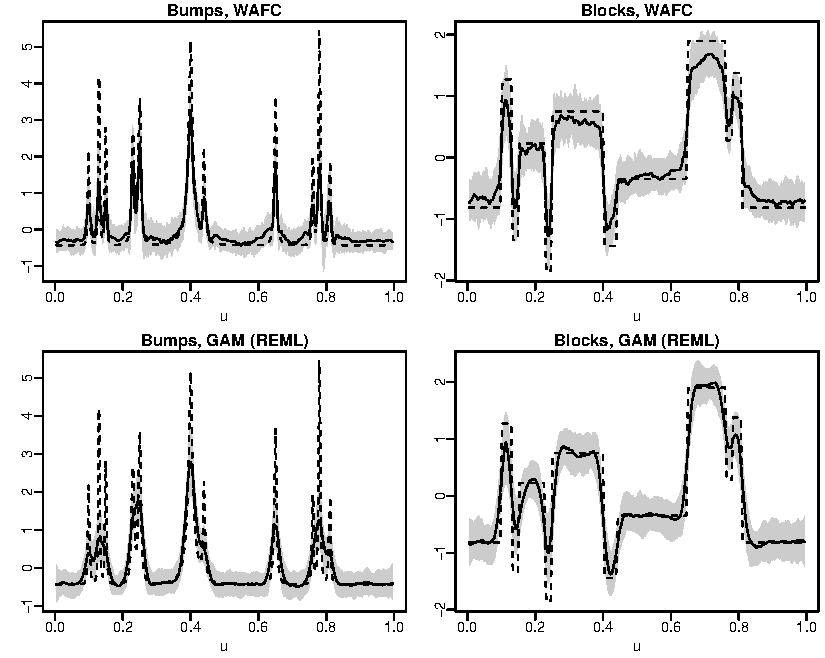
\includegraphics[width=\textwidth]{figures/sim-bands.pdf}
\caption{Simulation, inhomogeneous cell, $n = 1000$, the components of
Figure 1 of the paper: the pointwise median (solid line) and the 5\% and
95\% quantiles (band) over the 100 replicates of the WAFC (top) and of GAM
(REML) (bottom), with the truth (dashed line).}
\label{fig:sim-bands}
\end{figure}



% E5b (k = 6): as tabelas da S9 nao passam para a S10.
\clearpage

%%%%%%%%%%%%%%%%%%%%%%%%%%%%%%%%%%%%%%%%%%%%%%%%%%%%%%%%%%%%%%%%%%%%%%%%%%%%%%
% E5h (k = 5): a S10, o que completa a Secao 6 do ms_5 e a segunda aplicacao
% (D57: beijing.heat no supp, com tabela e figura). Os dados e o modelo sao os de
% wafc-studies/R/application_data.R e data/README.md; o paragrafo da temporada e
% o rascunho da L13 (ESTADO.md), com "neighbouring" fora; as marcas sao as
% nominais (D66). E5k (2026-10-08): os marcadores [E6.2] trocados pelos numeros de
% results/tables/ (prediction-, structure-, choices- e readings-<app>.csv; cada um e a
% sua coluna no handoff-E5k.md); a frase da grade da E6.2b (D76(c)), com o escopo da
% sondagem (as particoes 1 a 3 nos splines, o ajuste inteiro no WAFC); a frase das
% tabelas casada com o que o application_prediction() calcula (a diferenca e o wins
% contra o spline de menor erro medio, nao contra o melhor de cada particao).

